% Compiles with IEEEtran (Overleaf) when available; otherwise falls back to an IEEE-like article layout.
\IfFileExists{IEEEtran.cls}
  {\documentclass[conference]{IEEEtran}\newif\ifieee\ieeetrue}
  {\documentclass[10pt,twocolumn]{article}\newif\ifieee\ieeefalse}

\ifieee\else
  \usepackage[letterpaper,top=0.75in,bottom=1in,left=0.625in,right=0.625in,columnsep=0.25in]{geometry}
  
  \usepackage{titlesec}
  \renewcommand\thesection{\Roman{section}}
  \renewcommand\thesubsection{\Alph{subsection}}
  \titleformat{\section}{\centering\normalsize\scshape}{\thesection.}{0.5em}{}
  \titleformat{\subsection}{\normalsize\itshape}{\thesubsection.}{0.5em}{}
  \titlespacing*{\section}{0pt}{1.6ex}{0.8ex}
  \titlespacing*{\subsection}{0pt}{1.2ex}{0.5ex}
  \usepackage[labelsep=period,font=footnotesize]{caption}
  \captionsetup[table]{labelformat=simple,name=TABLE,textfont=sc,justification=centering}
  \renewcommand\thetable{\Roman{table}}
  \captionsetup[figure]{name=Fig.}
  \pagestyle{plain}
  \setlength{\parindent}{1em}
  \newcommand{\IEEEauthorblockN}[1]{#1\\}
  \newcommand{\IEEEauthorblockA}[1]{{\small\itshape #1}}
  \newenvironment{IEEEkeywords}{\noindent\bfseries\itshape Index Terms---\normalfont\bfseries}{\par}
  \renewenvironment{abstract}{\noindent\bfseries\itshape Abstract---\normalfont\bfseries}{\par\medskip}
  \makeatletter\renewcommand\@maketitle{\begin{center}{\LARGE\@title\par}\vskip1.2em{\large\@author\par}\end{center}\vskip1em}\makeatother
\fi

\usepackage{amsmath,amssymb}
\ifieee\else\usepackage{txfonts}\fi
\usepackage{booktabs,tabularx,multirow}
\usepackage{tikz}
\usetikzlibrary{arrows.meta,positioning}
\usepackage{microtype}
\usepackage{enumitem}
\setlist{nosep,leftmargin=*}
\usepackage{xcolor}
\usepackage[hidelinks]{hyperref}

% self-explanatory variable names: V{NAME}
\newcommand{\V}[1]{\text{\small\sffamily\bfseries #1}}
\newcommand{\Vt}[1]{{\small\sffamily\bfseries #1}}
% all displayed formulas in bold, with extra line spacing for legibility
\everydisplay\expandafter{\the\everydisplay\boldmath}
\setlength{\jot}{5pt}
\allowdisplaybreaks

\begin{document}

\twocolumn[{%
\begin{center}
  {\LARGE\bfseries Worldwide Location--Inventory Optimisation of\\[2pt]
  Snakebite Antivenom Stockrooms from Open Geospatial Data\par}
  \vspace{10pt}
  {\normalsize
    Anto Rishath$^{1}$,\; Antonio Roger$^{1}$,\;
    Adarsh Pradeep$^{1}$,\; Naresh Kumar V$^{1}$\par}
  \vspace{4pt}
  {\small $^{1}$\textit{Amrita School of Artificial Intelligence,
    Amrita Vishwa Vidyapeetham, Coimbatore, India}\\
  \{cb.sc.u4aie23103, cb.sc.u4aie23104, cb.sc.u4aie23109,
    cb.sc.u4aie23165\}@cb.students.amrita.edu\par}
  \vspace{8pt}
\end{center}}]

\begin{abstract}
Snakebite envenoming kills an estimated 81{,}000--138{,}000 people every year, mostly in rural districts that are far from a reliable antivenom supply. This paper presents a reproducible, worldwide pipeline that converts open data into district-level antivenom demand and then into stockroom locations and vial stock levels for each country. WHO species range polygons, WHO district boundaries, WorldPop 2020 rasters, the Census of India 2011, the WHO antivenom catalogue and GBD 2019 mortality are fused across 41{,}053 districts in 206 countries. Expected treatment courses are allocated to districts in proportion to the rural population living inside medically important species ranges. A product-portfolio integer program selects antivenoms that neutralise the local species. A $p$-median model places stockroom hubs so that course-weighted resupply time is minimised. Each problem is solved to proven optimality, or to a certified gap, by Lagrangian relaxation, exact candidate elimination and a mixed-integer program. Hub stock levels follow an $(R,S)$ policy with exact compound-Poisson quantiles. A post-location allocation model rations limited supply, protects a national reserve of at least 8\% of demand and sizes capacity headroom for single-hub failure (N$-$1). Of 148 countries with a mortality anchor, 142 are solved to proven optimality and 6 have certified gaps of at most 1.9\%. In India, eight hubs need 3.37~million vials per replenishment cycle, and 119.5\% of designed capacity is required to keep a 99\% fill rate when any single hub fails.
\end{abstract}

\begin{IEEEkeywords}
Facility location, $p$-median, Lagrangian relaxation, inventory optimisation, compound Poisson, snakebite, antivenom, geospatial data fusion.
\end{IEEEkeywords}

\section{Introduction}
Antivenom is the only specific treatment for snakebite envenoming, yet supply is fragmented~\cite{who}. Products are species-specific, have short shelf lives and need a cold chain. Most deaths occur in rural South Asia and sub-Saharan Africa, where the distance to stock decides the outcome. Planning is difficult because district-level demand data are unavailable in most countries, the right product depends on the species found in each district, and both the network design and the stock levels have to be justified to health authorities.

This work treats the problem as a two-stage Operations Research (OR) model built only on open data. Stage one estimates demand: every district receives an expected number of antivenom courses per year, split by species. Stage two optimises the supply network for each country: it chooses the product portfolio, places $P$ stockroom hubs, sets stock levels and rations stock when supply or storage is short. The contributions are:
\begin{itemize}
\item A documented data pipeline that links WHO, WorldPop, Census and GBD sources at district level for 206 countries, with every parameter labelled \emph{observed}, \emph{calibrated} or \emph{assumption}.
\item An exact location solver that certifies optimality with a Lagrangian lower bound for every country, including instances with more than 5{,}000 districts.
\item An inventory and allocation layer that uses exact compound-Poisson demand, provably optimal rationing, a national reserve rule and N$-$1 capacity sizing.
\end{itemize}
Fig.~\ref{fig:flow} shows the full flow from raw data to the dashboard.

\begin{figure}[t]
\centering
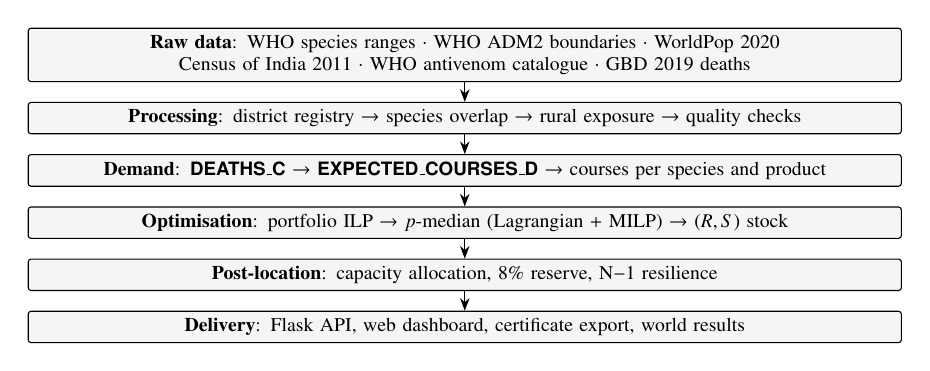
\begin{tikzpicture}[node distance=2.5mm, every node/.style={font=\scriptsize, align=center},
  box/.style={draw, rounded corners=1pt, text width=0.9\columnwidth, inner sep=2.5pt, fill=gray!8},
  arr/.style={-{Stealth[length=1.6mm]}}]
\node[box] (a) {\textbf{Raw data}: WHO species ranges $\cdot$ WHO ADM2 boundaries $\cdot$ WorldPop 2020\\ Census of India 2011 $\cdot$ WHO antivenom catalogue $\cdot$ GBD 2019 deaths};
\node[box, below=of a] (b) {\textbf{Processing}: district registry $\rightarrow$ species overlap $\rightarrow$ rural exposure $\rightarrow$ quality checks};
\node[box, below=of b] (c) {\textbf{Demand}: {\sffamily\bfseries DEATHS\_C} $\rightarrow$ {\sffamily\bfseries EXPECTED\_COURSES\_D} $\rightarrow$ courses per species and product};
\node[box, below=of c] (d) {\textbf{Optimisation}: portfolio ILP $\rightarrow$ $p$-median (Lagrangian + MILP) $\rightarrow$ $(R,S)$ stock};
\node[box, below=of d] (e) {\textbf{Post-location}: capacity allocation, 8\% reserve, N$-$1 resilience};
\node[box, below=of e] (f) {\textbf{Delivery}: Flask API, web dashboard, certificate export, world results};
\foreach \x/\y in {a/b,b/c,c/d,d/e,e/f} \draw[arr] (\x) -- (\y);
\end{tikzpicture}
\caption{End-to-end pipeline from open data to certified stockroom plans.}
\label{fig:flow}
\end{figure}

\section{Data Sources}
Table~\ref{tab:sources} lists all inputs~\cite{whosnb,gbd,worldpop,census}. Each source is public and downloaded by one script (\Vt{fetch\_global\_inputs.sh}). No value is imputed silently: a missing value either raises an error or is flagged in the output.

\begin{table}[t]
\caption{Data Sources}
\label{tab:sources}
\centering\footnotesize
\begin{tabularx}{\columnwidth}{@{}lXl@{}}
\toprule
Source & Content used & Role \\
\midrule
WHO SNBPROD layer 1 & Species range polygons, category code (Cat-1/Cat-2) & Presence \\
WHO SNBPROD layer 2 & Species master: names, family, regions & Metadata \\
WHO SNBPROD table 6 & Antivenom products, species links, specificity & Portfolio \\
WHO Detailed ADM2 & District (ADM2) boundary polygons & Registry \\
WorldPop 2020 & 1 km UN-adjusted population rasters & Exposure \\
Census of India 2011 & Population, rural households, agricultural workers & Exposure (IND) \\
DataMeet 2011 & Census district boundaries & Interpolation \\
GeoNames cities500 & Settlements $\geq$500 people & Fallback \\
IHME GBD 2019 & Snakebite deaths per country (via OWID) & Demand anchor \\
\bottomrule
\end{tabularx}
\end{table}

\section{Data Collection}
WHO layers are queried from the ArcGIS REST service in pages of 1{,}000 features and saved as GeoJSON per country. WorldPop rasters are downloaded per ISO3 code. The downloads run in parallel with four workers, because the WHO server resets connections above that rate. Each file is checked after download: empty or truncated GeoJSON files (for example, the first Paraguay file) are fetched again. The Census of India tables and DataMeet boundaries are joined on the 2011 census district code. GBD 2019 deaths are read from the Our World in Data export, which gives one value per country and year.

\section{Data Processing}
\subsection{District Registry}
Each WHO ADM2 polygon becomes one district with the key \Vt{DISTRICT\_ID} $=$ \Vt{ISO3$\,|\,$ADM1$\,|\,$ADM2}. Duplicate keys are dissolved into one geometry. All areas and overlaps are computed in the equal-area projection EPSG:6933 so that \Vt{AREA\_KM2\_D} is not distorted at high latitude. The registry holds 41{,}053 districts in 206 countries and six WHO regions.

\subsection{Species Presence}
Range polygons are dissolved per species, because the WHO layer stores one species in many pieces with region-specific categories. For district $d$ and species $s$,
\begin{equation}
\V{OVERLAP\_FRAC\_DS} = \frac{\text{area}\,(\V{DISTRICT\_D} \cap \V{RANGE\_S})}{\V{AREA\_KM2\_D}}
\end{equation}
Pairs with $\V{OVERLAP\_FRAC\_DS} < 0.001$ are removed as boundary slivers. A pair is tagged Category~1 if at least 0.1\% of the district lies inside the Cat-1 part of the range. When a district has no polygon, its centroid is tested instead. The result is 213{,}271 district--species pairs for 372 species (Table~\ref{tab:processed}).

\subsection{Population and Exposure}
The vulnerable group is the rural population that lives where medically important snakes live. For WorldPop countries, raster cells are summed inside each district polygon. A cell is rural when its density is below the urban-centre threshold of 1{,}500 people/km$^2$ from the UN Degree of Urbanisation~\cite{degurba}. Then
\begin{align}
&\V{VULNERABLE\_POPULATION\_D} = \sum_{\V{CELL}\in\V{RANGE\_CELLS\_D}}\nonumber\\
&\qquad\qquad \V{RURAL\_POPULATION\_CELL}
\end{align}
where \Vt{RANGE\_CELLS\_D} is the set of cells of district \Vt{D} that lie inside at least one species range.
For India, census values are moved from 2011 census districts to WHO districts by areal interpolation. The exposure base is \Vt{AGRICULTURAL\_WORKERS\_D} inside species ranges, because farm work is the main risk factor there. Where no raster is available, GeoNames settlements are used and the district is flagged \emph{provisional}, since this source undercounts villages.

\subsection{Antivenom Catalogue}
The WHO product table gives 713 product--species links for 120 products from 51 manufacturers. Each link has a specificity class, which is mapped to a quality weight: immunising species 1.0, published paraspecificity 0.8, label claim 0.6 and legacy complex 0.5. A product that is not registered in the country gets a factor of 0.9, because it must be imported.

\subsection{Quality Checks}
Automated checks run after each stage: unique keys, overlap fractions in $[0,1]$, non-negative populations, national population against UN totals, and exact demand conservation (the sum of district courses must equal the national total). The Canada run failed this last check, which exposed districts with exposure but no species rows. The fix sets exposure to zero in such districts.

\begin{table}[t]
\caption{Processed Dataset Summary}
\label{tab:processed}
\centering\footnotesize
\begin{tabularx}{\columnwidth}{@{}Xr@{}}
\toprule
Item & Value \\
\midrule
Districts / countries & 41{,}053 / 206 \\
\quad presence by polygon / centroid / none & 31{,}696 / 9{,}103 / 254 \\
District--species pairs (Cat-1 / Cat-2) & 91{,}937 / 121{,}334 \\
Species with range data & 372 \\
Population source: WorldPop / Census / GeoNames & 30{,}883 / 813 / 9{,}357 \\
Total / rural population (billion) & 7.49 / 4.20 \\
\Vt{VULNERABLE\_POPULATION} (billion) & 3.48 \\
Antivenom products / manufacturers / links & 120 / 51 / 713 \\
\bottomrule
\end{tabularx}
\end{table}

\section{Demand Model}
Country deaths are scaled to envenomings with one global ratio. The WHO reports 1.8--2.7~M envenomings and 81{,}000--138{,}000 deaths per year, so the midpoint ratio is $\V{ENVENOMINGS\_PER\_DEATH} = 20.5$ (scenarios 13 and 35.5). A share $\V{P\_ANTIVENOM} = 0.75$ of envenomings need antivenom. The district demand is
\begin{align}
&\V{EXPECTED\_COURSES\_D} = \V{DEATHS\_C}\nonumber\\
&\qquad \times \V{ENVENOMINGS\_PER\_DEATH}\nonumber\\
&\qquad \times \V{P\_ANTIVENOM}\times\V{EXPOSURE\_SHARE\_D}
\end{align}
where
\begin{align}
&\V{EXPOSURE\_SHARE\_D}\nonumber\\
&\qquad = \frac{\V{VULNERABLE\_POPULATION\_D}}{\sum_{\V{D}\in\V{C}}\V{VULNERABLE\_POPULATION\_D}}
\end{align}
District courses are split between species by overlap and category:
\begin{align}
&\V{COURSES\_DS} = \V{EXPECTED\_COURSES\_D}\times\frac{\V{RISK\_DS}}{\sum_{\V{S}}\V{RISK\_DS}}\\
&\V{RISK\_DS} = \V{OVERLAP\_FRAC\_DS}\nonumber\\
&\qquad\times\V{CATEGORY\_WEIGHT\_DS}
\end{align}
with weight 1 for Cat-1 and 0.1 for Cat-2. The split changes only the product mix, never the district total.

A course uses $\V{VIALS\_PER\_COURSE} \in \{10, 20\}$ vials: 10 vials, plus a repeat dose with probability 0.3. The mean is 13 vials per course.

\section{Optimisation Model}
\subsection{Product Portfolio}
For each country, a binary program selects the products to stock. Let \Vt{USE\_PRODUCT\_K} open product $k$ and \Vt{COVER\_SK} assign species $s$ to product $k$:
\begin{align}
\max\;\; & \sum_{\V{S},\V{K}}\V{COURSES\_S}\times\V{QUALITY\_SK}\times\V{COVER\_SK}\nonumber\\
&\quad - \epsilon\sum_{\V{K}}\V{USE\_PRODUCT\_K}\\
\text{s.t.}\;\; & \sum_{\V{K}}\V{COVER\_SK} \le 1 \qquad \forall\,\V{S}\\
& \V{COVER\_SK} \le \V{USE\_PRODUCT\_K} \qquad \forall\,\V{S},\V{K}
\end{align}
where \Vt{QUALITY\_SK} is the specificity weight times the registration factor, and $\epsilon=10^{-6}$ prefers fewer products when quality ties. Courses of species with no effective product are reported separately as \Vt{COURSES\_NO\_EFFECTIVE\_ANTIVENOM}.

\subsection{Hub Location}
Every district centroid is a candidate site $j$. Road travel time is estimated as
\begin{equation}
\V{TRAVEL\_HOURS\_DJ} = \frac{1.35\times\V{HAVERSINE\_KM\_DJ}}{40\ \text{km/h}}
\end{equation}
where 1.35 is a national road circuity factor~\cite{ballou}. With binary \Vt{HUB\_OPEN\_J} and \Vt{ASSIGN\_DJ}, the $p$-median model~\cite{hakimi} is
\begin{align}
\min\;\; & \sum_{\V{D},\V{J}}\V{EXPECTED\_COURSES\_D}\nonumber\\
&\quad\times\V{TRAVEL\_HOURS\_DJ}\times\V{ASSIGN\_DJ}\label{eq:pm}\\
\text{s.t.}\;\; & \sum_{\V{J}} \V{ASSIGN\_DJ} = 1 \qquad \forall\,\V{D}\\
& \V{ASSIGN\_DJ} \le \V{HUB\_OPEN\_J} \qquad \forall\,\V{D},\V{J}\\
& \sum_{\V{J}} \V{HUB\_OPEN\_J} = \V{NUM\_HUBS}\\
& \V{ASSIGN\_DJ},\ \V{HUB\_OPEN\_J} \in \{0,1\}
\end{align}
The objective is total course-hours per year, so hubs move toward districts with high demand. In the world run the number of hubs is
\begin{equation}
\V{NUM\_HUBS} = \min\bigl(20,\ \mathrm{round}(\sqrt{\V{NUM\_DISTRICTS}}\,/\,2)\bigr)
\end{equation}
the dashboard lets the user change it and shows the trade-off curve.

\subsection{Solution Method}
A greedy start improved by Teitz--Bart vertex swaps~\cite{teitz} gives an upper bound \Vt{UB}. The assignment constraints are relaxed with multipliers \Vt{LAMBDA\_D}. For each site, the reduced cost is
\begin{align}
\V{RHO\_J} = \sum_{\V{D}} \min\bigl(0,\ & \V{EXPECTED\_COURSES\_D}\nonumber\\
&\times\V{TRAVEL\_HOURS\_DJ}\nonumber\\
&- \V{LAMBDA\_D}\bigr)
\end{align}
and the lower bound is
\begin{equation}
\V{LB} = \sum_{\V{D}}\V{LAMBDA\_D} + \!\!\sum_{\substack{\V{NUM\_HUBS}\\ \text{smallest}}}\!\! \V{RHO\_J}
\end{equation} Subgradient steps maximise \Vt{LB}~\cite{hwc,beasley}. If \Vt{LB} reaches \Vt{UB}, the incumbent is optimal. Otherwise, a site $j$ is closed exactly when
\begin{equation}
\V{LB} - \V{RHO\_PTH\_SMALLEST} + \V{RHO\_J} > \V{UB}
\end{equation}
where \Vt{RHO\_PTH\_SMALLEST} is the \Vt{NUM\_HUBS}-th smallest reduced cost. This removes most candidates. The remaining model is solved by HiGHS~\cite{highs}. The reported gap, $(\V{UB}-\V{LB})/\V{UB}$, is therefore a proven bound on the distance from the optimum.

\subsection{Stock Levels}
Each hub $h$ follows an $(R,S)$ policy~\cite{axsater} with review period $R=3$ months and lead time $L=1$ month. The demand for product $k$ over $R+L$ is compound Poisson: course arrivals are Poisson with mean
\begin{equation}
\V{MEAN\_COURSES\_CYCLE\_HK} = \V{COURSES\_HK}\times\frac{R+L}{12}
\end{equation}
and each course needs 10 or 20 vials. By Poisson splitting, the vial demand is $10\,(N_1 + 2N_2)$ with independent Poisson $N_1, N_2$. Its exact distribution is computed by FFT convolution. The order-up-to level is the smallest stock that meets the cycle service level $\alpha = 0.99$:
\begin{align}
\V{STOCK\_LEVEL\_HK} = \min\bigl\{\,S :\ & \Pr(\V{CYCLE\_DEMAND\_HK} \le S)\nonumber\\
& \ge 0.99\,\bigr\}
\end{align}

\subsection{Capacity Allocation and Reserve}
After locations are fixed, the designed stock $\V{DESIGNED\_CAPACITY\_H} = \sum_k \V{STOCK\_LEVEL\_HK}$ becomes the ground truth. The user scales it by \Vt{CAPACITY\_PCT} and limits supply by \Vt{SUPPLY\_PCT}. Districts are routed to hubs by a capacitated transport LP, with safety stock updated in a fixed point. Vials are then rationed:
\begin{align}
\max\;\; & \sum_{\V{H},\V{K}}\V{VIALS\_SERVED\_HK}\\
\text{s.t.}\;\; & \sum_{\V{K}} \V{ALLOC\_VIALS\_HK} \le \V{HUB\_CAPACITY\_H}\\
& \sum_{\V{H},\V{K}}\V{ALLOC\_VIALS\_HK} \le \V{NATIONAL\_SUPPLY}\\
& \sum_{\V{K}} \V{ALLOC\_VIALS\_HK} \ge \V{RESERVE\_FLOOR\_H}
\end{align}
where the expected number of vials actually used is
\begin{align}
\V{VIALS\_SERVED\_HK} = \mathbb{E}\bigl[\min(&\V{CYCLE\_DEMAND\_HK},\nonumber\\
&\V{ALLOC\_VIALS\_HK})\bigr]
\end{align}
The reserve rule fixes a pool equal to 8\% of national need, shared equally by hubs and capped at each hub's own target:
\begin{align}
\V{RESERVE\_SHARE} &= \frac{0.08\times\sum_{\V{H}}\V{TARGET\_VIALS\_H}}{\V{NUM\_HUBS}}\\
\V{RESERVE\_FLOOR\_H} &= \min(\V{TARGET\_VIALS\_H},\nonumber\\
&\qquad\quad \V{RESERVE\_SHARE})
\end{align}
This keeps stock at low-demand (dormant) hubs. The marginal gain of one more batch of $g$ vials is $g\cdot\Pr(\V{CYCLE\_DEMAND\_HK} > a)$, which falls as $a$ grows. The objective is therefore separable and concave, and the hub limits are nested inside the national limit (a laminar family). In this case, greedy allocation by largest marginal gain is optimal~\cite{fed}.

\subsection{N$-$1 Resilience}
For each hub $f$, the hub is removed and its districts are routed to the surviving hubs. Bisection finds the smallest \Vt{CAPACITY\_PCT} at which the network fill rate stays at least 0.99. The largest value over all $f$ is the capacity headroom that survives any single-hub failure.

\section{Results}
\subsection{Worldwide Solution Quality}
Countries with both a GBD anchor and species data are solved one by one (Table~\ref{tab:world}). All 148 instances return a certificate. In 111 cases the Lagrangian bound alone closes the gap; in 31 more HiGHS proves optimality. Six large instances (Brazil, Colombia, Japan, Mexico, Romania, USA) end with certified gaps of 0.6--1.9\%. The greedy plus Teitz--Bart heuristic reaches the optimum in 94 of 147 countries but is up to 9.0\% worse in the remaining cases, so the exact bound is needed to confirm optimality.

\begin{table}[t]
\caption{Worldwide Results (Default Parameters)}
\label{tab:world}
\centering\footnotesize
\begin{tabularx}{\columnwidth}{@{}Xr@{}}
\toprule
Metric & Value \\
\midrule
Countries solved & 148 \\
\quad proven optimal / certified gap & 142 / 6 \\
\quad largest certified gap & 1.87\% (MEX) \\
Heuristic matches optimum & 94 of 147 \\
\quad maximum / mean heuristic excess & 9.0\% / 0.5\% \\
Total solve time / slowest country & 928 s / 508 s (BRA) \\
Hubs opened (excl.\ CAN) & 824 \\
\Vt{EXPECTED\_COURSES} per year & 0.93 M \\
\Vt{COURSES\_NO\_EFFECTIVE\_ANTIVENOM} & 40{,}751 (4.4\%) \\
Vials stocked (one cycle) & 4.34 M \\
Courses within 8 h of a hub & 85.5\% \\
\bottomrule
\end{tabularx}
\end{table}

India carries 82\% of the modelled courses (763{,}732 per year from 51{,}100 GBD deaths). Table~\ref{tab:top} shows the largest burdens. Countries with dense district grids and good roads (Bangladesh, Nigeria, Kenya) keep almost all courses within 8~h. Large countries with few hubs (India, DR Congo) do not.

\begin{table}[t]
\caption{Largest National Burdens}
\label{tab:top}
\centering\footnotesize
\setlength{\tabcolsep}{3.5pt}
\begin{tabular}{@{}lrrrrrr@{}}
\toprule
ISO3 & Districts & Hubs & Courses/yr & Vials & Mean h & $\le$8 h \% \\
\midrule
IND & 813 & 14 & 763{,}732 & 3{,}384{,}870 & 5.58 & 83.4 \\
PAK & 151 & 6 & 31{,}530 & 147{,}020 & 3.61 & 97.3 \\
NGA & 774 & 14 & 21{,}147 & 107{,}580 & 2.92 & 99.7 \\
BGD & 64 & 4 & 12{,}357 & 60{,}730 & 2.54 & 100.0 \\
COD & 519 & 11 & 7{,}807 & 40{,}050 & 4.99 & 84.3 \\
ETH & 109 & 5 & 7{,}377 & 38{,}550 & 4.60 & 88.3 \\
KEN & 316 & 9 & 4{,}721 & 26{,}730 & 2.19 & 98.6 \\
\bottomrule
\end{tabular}
\end{table}

\subsection{India Case Study (Eight Hubs)}
With $\V{NUM\_HUBS}=8$, the subgradient method closes the gap in 524 iterations and eliminates 803 of 813 candidate sites; the full solve takes 0.94~s. The portfolio has six products, including the Indian polyvalent serum raised against the ``big four'' species. Table~\ref{tab:india} shows the designed hubs and the allocation when supply is cut to 80\% with an 8\% reserve. Every hub keeps at least its reserve floor of about 33{,}650 vials. The greedy rule sends scarce vials to the highest-risk hub (Jamui, 94\% fill) and away from hubs with flatter demand. The network fill rate falls to 81.4\% under the 20\% supply cut.

\begin{table}[t]
\caption{India: Designed Stock and Allocation at 80\% Supply}
\label{tab:india}
\centering\footnotesize
\setlength{\tabcolsep}{3.5pt}
\begin{tabular}{@{}lrrrr@{}}
\toprule
Hub (state) & Pop. (M) & Designed & Allocated & Fill \\
\midrule
Jamui (BR) & 226.8 & 616{,}520 & 570{,}700 & 0.94 \\
Bidar (KA) & 141.3 & 502{,}280 & 407{,}280 & 0.82 \\
Amethi (UP) & 165.1 & 491{,}500 & 345{,}500 & 0.71 \\
Dahod (GJ) & 157.6 & 478{,}870 & 326{,}020 & 0.69 \\
South-West (DL) & 210.8 & 448{,}030 & 397{,}520 & 0.90 \\
Gariaband (CG) & 98.5 & 376{,}820 & 318{,}670 & 0.86 \\
Dharmapuri (TN) & 155.1 & 335{,}500 & 232{,}190 & 0.70 \\
Marigoan (AS) & 49.7 & 117{,}340 & 95{,}600 & 0.85 \\
\midrule
Total & 1{,}204.9 & 3{,}366{,}860 & 2{,}693{,}480 & 0.81 \\
\bottomrule
\end{tabular}
\end{table}

\subsection{Single-Hub Failure}
Table~\ref{tab:n1} gives the N$-$1 results with full supply and the 8\% reserve. At 100\% capacity, losing Jamui drops the fill rate to 0.83 and reroutes 20.9\% of courses. Keeping a 0.99 fill rate under any single failure needs 119.5\% of designed capacity. This is the basis for setting the dashboard capacity slider up to 150\%.

\begin{table}[t]
\caption{India N$-$1 Resilience (Eight Hubs)}
\label{tab:n1}
\centering\footnotesize
\begin{tabular}{@{}lrrr@{}}
\toprule
Failed hub & Rerouted \% & Fill at 100\% & Capacity \% needed \\
\midrule
Jamui & 20.9 & 0.831 & 119.5 \\
Dahod & 13.6 & 0.873 & 115.4 \\
Bidar & 14.5 & 0.866 & 114.8 \\
Amethi & 13.7 & 0.869 & 114.3 \\
South-West & 14.5 & 0.882 & 112.5 \\
Gariaband & 6.5 & 0.904 & 110.2 \\
Dharmapuri & 15.1 & 0.916 & 108.4 \\
Marigoan & 5.3 & 0.982 & 102.5 \\
\bottomrule
\end{tabular}
\end{table}

\subsection{Verification}
The code base has 74 automated tests. They check that: the compound-Poisson distribution has mean $\mu\,\mathbb{E}[V]$ and variance $\mu\,\mathbb{E}[V^2]$; the quantile matches 400{,}000 Monte Carlo draws; greedy rationing equals brute-force search, also with nested hub and national limits; the $p$-median solution equals brute force on small instances; more hubs never increase the objective; and district courses sum exactly to the national total. API tests confirm that India's population is 1.15--1.25~billion, that every stock level meets $\alpha = 0.99$, and that disabling a hub never lowers resupply time.

\section{Limitations}
\begin{itemize}
\item \textbf{Travel time.} Haversine distance times a circuity factor ignores terrain, roads and water. Island districts such as Nicobar are assigned across the sea and should be handled as separate networks.
\item \textbf{Demand.} One global envenoming-to-death ratio implies one case fatality rate; the true rate is higher where care is poor. GBD 2019 deaths, Census 2011 counts and WorldPop 2020 also differ in year.
\item \textbf{Population.} 9{,}357 districts in Canada, Mexico, Philippines, Romania, Thailand and Vietnam use GeoNames and are flagged provisional until WorldPop rasters are added.
\item \textbf{Ranges.} WHO range maps are coarse, and 9{,}103 districts rely on a centroid test.
\item \textbf{Parameters.} Dose, repeat rate, review period and speed are planning assumptions and are covered by scenario runs rather than measured values.
\end{itemize}

\section{Conclusion}
In this work, antivenom supply plans are built for 148 countries using only open data. District demand follows the rural population that lives inside medically important species ranges. Hubs are placed by an exact $p$-median model with a certified bound, and stock levels come from exact compound-Poisson quantiles. The allocation layer shows what happens when storage or supply is short: high-risk hubs are served first, every hub keeps an 8\% national reserve share, and the capacity needed to survive one hub failure is computed explicitly. The next steps are road-network travel times, WorldPop coverage for the provisional countries, and sub-national validation against hospital antivenom records.

\begin{thebibliography}{10}
\footnotesize
\bibitem{who} World Health Organization, ``Snakebite envenoming,'' Fact sheet, Geneva, Switzerland, 2023.
\bibitem{whosnb} World Health Organization, ``Snakebite information and data platform,'' 2023. [Online]. Available: https://snbdatainfo.who.int
\bibitem{gbd} GBD 2019 Snakebite Envenomation Collaborators, ``Global mortality of snakebite envenoming between 1990 and 2019,'' \emph{Nat. Commun.}, vol. 13, art. 6160, 2022.
\bibitem{worldpop} WorldPop, ``Global high resolution population denominators project,'' Univ. Southampton, 2020, doi: 10.5258/SOTON/WP00671.
\bibitem{census} Office of the Registrar General and Census Commissioner, \emph{Census of India 2011: Primary Census Abstract}. New Delhi, India, 2011.
\bibitem{degurba} European Commission \emph{et al.}, \emph{Applying the Degree of Urbanisation}. Luxembourg: Publications Office of the EU, 2021.
\bibitem{hakimi} S. L. Hakimi, ``Optimum locations of switching centers and the absolute centers and medians of a graph,'' \emph{Oper. Res.}, vol. 12, no. 3, pp. 450--459, 1964.
\bibitem{teitz} M. B. Teitz and P. Bart, ``Heuristic methods for estimating the generalized vertex median of a weighted graph,'' \emph{Oper. Res.}, vol. 16, no. 5, pp. 955--961, 1968.
\bibitem{beasley} J. E. Beasley, ``Lagrangean heuristics for location problems,'' \emph{Eur. J. Oper. Res.}, vol. 65, no. 3, pp. 383--399, 1993.
\bibitem{hwc} M. Held, P. Wolfe, and H. P. Crowder, ``Validation of subgradient optimization,'' \emph{Math. Program.}, vol. 6, pp. 62--88, 1974.
\bibitem{highs} Q. Huangfu and J. A. J. Hall, ``Parallelizing the dual revised simplex method,'' \emph{Math. Program. Comput.}, vol. 10, pp. 119--142, 2018.
\bibitem{ballou} R. H. Ballou, H. Rahardja, and N. Sakai, ``Selected country circuity factors for road travel distance estimation,'' \emph{Transp. Res. A}, vol. 36, no. 9, pp. 843--848, 2002.
\bibitem{axsater} S. Axs\"ater, \emph{Inventory Control}, 3rd ed. Cham, Switzerland: Springer, 2015.
\bibitem{fed} A. Federgruen and H. Groenevelt, ``The greedy procedure for resource allocation problems: Necessary and sufficient conditions for optimality,'' \emph{Oper. Res.}, vol. 34, no. 6, pp. 909--918, 1986.
\end{thebibliography}

\end{document}
